% Options for packages loaded elsewhere
\PassOptionsToPackage{unicode}{hyperref}
\PassOptionsToPackage{hyphens}{url}
\PassOptionsToPackage{dvipsnames,svgnames,x11names}{xcolor}
%
\documentclass[
  12pt,
]{article}

\usepackage{amsmath,amssymb}
\usepackage{iftex}
\ifPDFTeX
  \usepackage[T1]{fontenc}
  \usepackage[utf8]{inputenc}
  \usepackage{textcomp} % provide euro and other symbols
\else % if luatex or xetex
  \usepackage{unicode-math}
  \defaultfontfeatures{Scale=MatchLowercase}
  \defaultfontfeatures[\rmfamily]{Ligatures=TeX,Scale=1}
\fi
\usepackage{lmodern}
\ifPDFTeX\else  
    % xetex/luatex font selection
\fi
% Use upquote if available, for straight quotes in verbatim environments
\IfFileExists{upquote.sty}{\usepackage{upquote}}{}
\IfFileExists{microtype.sty}{% use microtype if available
  \usepackage[]{microtype}
  \UseMicrotypeSet[protrusion]{basicmath} % disable protrusion for tt fonts
}{}
\makeatletter
\@ifundefined{KOMAClassName}{% if non-KOMA class
  \IfFileExists{parskip.sty}{%
    \usepackage{parskip}
  }{% else
    \setlength{\parindent}{0pt}
    \setlength{\parskip}{6pt plus 2pt minus 1pt}}
}{% if KOMA class
  \KOMAoptions{parskip=half}}
\makeatother
\usepackage{xcolor}
\usepackage[lmargin=1in,rmargin=1in,tmargin=1in,bmargin=1in]{geometry}
\setlength{\emergencystretch}{3em} % prevent overfull lines
\setcounter{secnumdepth}{3}
% Make \paragraph and \subparagraph free-standing
\ifx\paragraph\undefined\else
  \let\oldparagraph\paragraph
  \renewcommand{\paragraph}[1]{\oldparagraph{#1}\mbox{}}
\fi
\ifx\subparagraph\undefined\else
  \let\oldsubparagraph\subparagraph
  \renewcommand{\subparagraph}[1]{\oldsubparagraph{#1}\mbox{}}
\fi

\usepackage{color}
\usepackage{fancyvrb}
\newcommand{\VerbBar}{|}
\newcommand{\VERB}{\Verb[commandchars=\\\{\}]}
\DefineVerbatimEnvironment{Highlighting}{Verbatim}{commandchars=\\\{\}}
% Add ',fontsize=\small' for more characters per line
\usepackage{framed}
\definecolor{shadecolor}{RGB}{241,243,245}
\newenvironment{Shaded}{\begin{snugshade}}{\end{snugshade}}
\newcommand{\AlertTok}[1]{\textcolor[rgb]{0.68,0.00,0.00}{#1}}
\newcommand{\AnnotationTok}[1]{\textcolor[rgb]{0.37,0.37,0.37}{#1}}
\newcommand{\AttributeTok}[1]{\textcolor[rgb]{0.40,0.45,0.13}{#1}}
\newcommand{\BaseNTok}[1]{\textcolor[rgb]{0.68,0.00,0.00}{#1}}
\newcommand{\BuiltInTok}[1]{\textcolor[rgb]{0.00,0.23,0.31}{#1}}
\newcommand{\CharTok}[1]{\textcolor[rgb]{0.13,0.47,0.30}{#1}}
\newcommand{\CommentTok}[1]{\textcolor[rgb]{0.37,0.37,0.37}{#1}}
\newcommand{\CommentVarTok}[1]{\textcolor[rgb]{0.37,0.37,0.37}{\textit{#1}}}
\newcommand{\ConstantTok}[1]{\textcolor[rgb]{0.56,0.35,0.01}{#1}}
\newcommand{\ControlFlowTok}[1]{\textcolor[rgb]{0.00,0.23,0.31}{#1}}
\newcommand{\DataTypeTok}[1]{\textcolor[rgb]{0.68,0.00,0.00}{#1}}
\newcommand{\DecValTok}[1]{\textcolor[rgb]{0.68,0.00,0.00}{#1}}
\newcommand{\DocumentationTok}[1]{\textcolor[rgb]{0.37,0.37,0.37}{\textit{#1}}}
\newcommand{\ErrorTok}[1]{\textcolor[rgb]{0.68,0.00,0.00}{#1}}
\newcommand{\ExtensionTok}[1]{\textcolor[rgb]{0.00,0.23,0.31}{#1}}
\newcommand{\FloatTok}[1]{\textcolor[rgb]{0.68,0.00,0.00}{#1}}
\newcommand{\FunctionTok}[1]{\textcolor[rgb]{0.28,0.35,0.67}{#1}}
\newcommand{\ImportTok}[1]{\textcolor[rgb]{0.00,0.46,0.62}{#1}}
\newcommand{\InformationTok}[1]{\textcolor[rgb]{0.37,0.37,0.37}{#1}}
\newcommand{\KeywordTok}[1]{\textcolor[rgb]{0.00,0.23,0.31}{#1}}
\newcommand{\NormalTok}[1]{\textcolor[rgb]{0.00,0.23,0.31}{#1}}
\newcommand{\OperatorTok}[1]{\textcolor[rgb]{0.37,0.37,0.37}{#1}}
\newcommand{\OtherTok}[1]{\textcolor[rgb]{0.00,0.23,0.31}{#1}}
\newcommand{\PreprocessorTok}[1]{\textcolor[rgb]{0.68,0.00,0.00}{#1}}
\newcommand{\RegionMarkerTok}[1]{\textcolor[rgb]{0.00,0.23,0.31}{#1}}
\newcommand{\SpecialCharTok}[1]{\textcolor[rgb]{0.37,0.37,0.37}{#1}}
\newcommand{\SpecialStringTok}[1]{\textcolor[rgb]{0.13,0.47,0.30}{#1}}
\newcommand{\StringTok}[1]{\textcolor[rgb]{0.13,0.47,0.30}{#1}}
\newcommand{\VariableTok}[1]{\textcolor[rgb]{0.07,0.07,0.07}{#1}}
\newcommand{\VerbatimStringTok}[1]{\textcolor[rgb]{0.13,0.47,0.30}{#1}}
\newcommand{\WarningTok}[1]{\textcolor[rgb]{0.37,0.37,0.37}{\textit{#1}}}

\providecommand{\tightlist}{%
  \setlength{\itemsep}{0pt}\setlength{\parskip}{0pt}}\usepackage{longtable,booktabs,array}
\usepackage{calc} % for calculating minipage widths
% Correct order of tables after \paragraph or \subparagraph
\usepackage{etoolbox}
\makeatletter
\patchcmd\longtable{\par}{\if@noskipsec\mbox{}\fi\par}{}{}
\makeatother
% Allow footnotes in longtable head/foot
\IfFileExists{footnotehyper.sty}{\usepackage{footnotehyper}}{\usepackage{footnote}}
\makesavenoteenv{longtable}
\usepackage{graphicx}
\makeatletter
\def\maxwidth{\ifdim\Gin@nat@width>\linewidth\linewidth\else\Gin@nat@width\fi}
\def\maxheight{\ifdim\Gin@nat@height>\textheight\textheight\else\Gin@nat@height\fi}
\makeatother
% Scale images if necessary, so that they will not overflow the page
% margins by default, and it is still possible to overwrite the defaults
% using explicit options in \includegraphics[width, height, ...]{}
\setkeys{Gin}{width=\maxwidth,height=\maxheight,keepaspectratio}
% Set default figure placement to htbp
\makeatletter
\def\fps@figure{htbp}
\makeatother
% definitions for citeproc citations
\NewDocumentCommand\citeproctext{}{}
\NewDocumentCommand\citeproc{mm}{%
  \begingroup\def\citeproctext{#2}\cite{#1}\endgroup}
\makeatletter
 % allow citations to break across lines
 \let\@cite@ofmt\@firstofone
 % avoid brackets around text for \cite:
 \def\@biblabel#1{}
 \def\@cite#1#2{{#1\if@tempswa , #2\fi}}
\makeatother
\newlength{\cslhangindent}
\setlength{\cslhangindent}{1.5em}
\newlength{\csllabelwidth}
\setlength{\csllabelwidth}{3em}
\newenvironment{CSLReferences}[2] % #1 hanging-indent, #2 entry-spacing
 {\begin{list}{}{%
  \setlength{\itemindent}{0pt}
  \setlength{\leftmargin}{0pt}
  \setlength{\parsep}{0pt}
  % turn on hanging indent if param 1 is 1
  \ifodd #1
   \setlength{\leftmargin}{\cslhangindent}
   \setlength{\itemindent}{-1\cslhangindent}
  \fi
  % set entry spacing
  \setlength{\itemsep}{#2\baselineskip}}}
 {\end{list}}
\usepackage{calc}
\newcommand{\CSLBlock}[1]{\hfill\break\parbox[t]{\linewidth}{\strut\ignorespaces#1\strut}}
\newcommand{\CSLLeftMargin}[1]{\parbox[t]{\csllabelwidth}{\strut#1\strut}}
\newcommand{\CSLRightInline}[1]{\parbox[t]{\linewidth - \csllabelwidth}{\strut#1\strut}}
\newcommand{\CSLIndent}[1]{\hspace{\cslhangindent}#1}

\usepackage{lipsum}
\makeatletter
\@ifpackageloaded{caption}{}{\usepackage{caption}}
\AtBeginDocument{%
\ifdefined\contentsname
  \renewcommand*\contentsname{Table of contents}
\else
  \newcommand\contentsname{Table of contents}
\fi
\ifdefined\listfigurename
  \renewcommand*\listfigurename{List of Figures}
\else
  \newcommand\listfigurename{List of Figures}
\fi
\ifdefined\listtablename
  \renewcommand*\listtablename{List of Tables}
\else
  \newcommand\listtablename{List of Tables}
\fi
\ifdefined\figurename
  \renewcommand*\figurename{Figure}
\else
  \newcommand\figurename{Figure}
\fi
\ifdefined\tablename
  \renewcommand*\tablename{Table}
\else
  \newcommand\tablename{Table}
\fi
}
\@ifpackageloaded{float}{}{\usepackage{float}}
\floatstyle{ruled}
\@ifundefined{c@chapter}{\newfloat{codelisting}{h}{lop}}{\newfloat{codelisting}{h}{lop}[chapter]}
\floatname{codelisting}{Listing}
\newcommand*\listoflistings{\listof{codelisting}{List of Listings}}
\makeatother
\makeatletter
\makeatother
\makeatletter
\@ifpackageloaded{caption}{}{\usepackage{caption}}
\@ifpackageloaded{subcaption}{}{\usepackage{subcaption}}
\makeatother
\ifLuaTeX
  \usepackage{selnolig}  % disable illegal ligatures
\fi
\usepackage{bookmark}

\IfFileExists{xurl.sty}{\usepackage{xurl}}{} % add URL line breaks if available
\urlstyle{same} % disable monospaced font for URLs
\hypersetup{
  pdftitle={Simart Template},
  pdfauthor={Sarah Malloc; Eliza Dealloc},
  pdfkeywords={template, demo},
  colorlinks=true,
  linkcolor={blue},
  filecolor={Maroon},
  citecolor={Blue},
  urlcolor={Blue},
  pdfcreator={LaTeX via pandoc}}


\usepackage{datetime}
\usepackage{booktabs}
\usepackage{chngcntr}
\usepackage{apptools}
\AtAppendix{\counterwithin{table}{section}}
\AtAppendix{\counterwithin{figure}{section}}

\title{Simart Template}
\author{
Sarah Malloc\footnote{Corresponding Author}\\
An Organization\\
Boston\\
\href{mailto:sm@example.org}{sm@example.org}\and 
Eliza Dealloc\\
Another Affiliation\\
\\
}
\date{}
\begin{document}


\def\spacingset#1{\renewcommand{\baselinestretch}%
{#1}\small\normalsize} \spacingset{1}

%Ipsum lorem

\maketitle
\begin{abstract}
This document is a template demonstrating the Simart format. In addition
to few tips on how to use quarto for producing articles.
\end{abstract}
 
\vspace{.2in}

\textbf{\textit{Keyword: }}
    template, 
    demo 

\textbf{\textit{JEL: }}
    J11, 
    A1 

\thispagestyle{empty}
\clearpage\pagenumbering{arabic}
\newpage
\spacingset{1.2} % DON'T change the spacing!
\section{Introduction}\label{sec-intro}

This is a very simple template for the creation of academic articles. It
is based on the documentclass article. It has also been adapted so it
includes the information of authors, thank you note, corresponding
author information, etc. Using APA7th for citations.

It also provides a quick review of some of the options I learn to use to
create sections of interest. Just for fun, it also generates LIPSUM
text, to fill the rest of the text.

\section{Citing documents}\label{sec-cite}

There are two ways to cite documents. One is using standard author(year)
format, as well as a (author, year) format.

In the first case you use \texttt{@CameronTrivedi2013} to obtain Cameron
and Trivedi (2013).

In the second case you use \texttt{{[}@CameronTrivedi2013{]}} to obtain
(Cameron and Trivedi, 2013).

\section{Authors, Keywords, JEL codes}\label{authors-keywords-jel-codes}

The template has been prepared and coded so you include the email, name
of the one institution affiliation, and the city of that institution.
You can also incorporate the attribute of corresponding author. You
cannot have more than 1 affiliation.

\begin{Shaded}
\begin{Highlighting}[]
\SpecialStringTok{  {-} }\NormalTok{name: Jon Dean}
\NormalTok{    email: jdean@jdean.org}
\NormalTok{    affiliations: }
\SpecialStringTok{        {-} }\NormalTok{name: Jdean  }
\NormalTok{          city: Somewhere, NU}
\NormalTok{    attributes:}
\NormalTok{        corresponding: true }
\end{Highlighting}
\end{Shaded}

For Keywords and JEL codes you can simply use the following:

\begin{Shaded}
\begin{Highlighting}[]
\AnnotationTok{keywords:}\CommentTok{ [word1, word2, word3]}
\AnnotationTok{jelcodes:}\CommentTok{ [jel1, jel2, jel4]}
\end{Highlighting}
\end{Shaded}

Make sure that you use square brackets \texttt{{[}{]}} when listing the
keywords and jelcodes.

\section{Math}\label{math}

You can write math in-line using latex standard syntax. For example
\texttt{\$\textbackslash{}beta\$} would create \(\beta\).

To write longer equations you need to use \texttt{\$\$} before and after
the expression. I find it useful to start a new line to do so. As in the
following example:

\begin{Shaded}
\begin{Highlighting}[]
\SpecialStringTok{$$y = }\SpecialCharTok{\textbackslash{}beta}\SpecialStringTok{ X + }\SpecialCharTok{\textbackslash{}varepsilon}
\SpecialStringTok{$$}
\end{Highlighting}
\end{Shaded}

\[y = \beta X + \varepsilon
\]

For multiple equation formulas, it may be convinient to use
\texttt{\textbackslash{}begin\{aligned\}} and
\texttt{\textbackslash{}end\{aligned\}}.

\begin{Shaded}
\begin{Highlighting}[]
\SpecialStringTok{$$}
\KeywordTok{\textbackslash{}begin}\NormalTok{\{}\ExtensionTok{aligned}\NormalTok{\}}
\SpecialStringTok{y \&= }\SpecialCharTok{\textbackslash{}beta}\SpecialStringTok{ X + }\SpecialCharTok{\textbackslash{}varepsilon}\SpecialStringTok{ }\SpecialCharTok{\textbackslash{}\textbackslash{}}
\SpecialCharTok{\textbackslash{}varepsilon}\SpecialStringTok{ \&}\SpecialCharTok{\textbackslash{}sim}\SpecialStringTok{ N(0,}\SpecialCharTok{\textbackslash{}sigma}\SpecialStringTok{\^{}2)}
\KeywordTok{\textbackslash{}end}\NormalTok{\{}\ExtensionTok{aligned}\NormalTok{\}}
\SpecialStringTok{$$}
\end{Highlighting}
\end{Shaded}

\[
\begin{aligned}
y &= \beta X + \varepsilon \\
\varepsilon &\sim N(0,\sigma^2)
\end{aligned}
\]

These equations can be easily cross referenced using
\texttt{\{\#eq-something\}} after \texttt{\$\$}. Instead of something,
we just need a unique id to call to. For example:

\begin{Shaded}
\begin{Highlighting}[]
\SpecialStringTok{$$}
\KeywordTok{\textbackslash{}begin}\NormalTok{\{}\ExtensionTok{aligned}\NormalTok{\}}
\SpecialStringTok{y \&= }\SpecialCharTok{\textbackslash{}beta}\SpecialStringTok{ X + }\SpecialCharTok{\textbackslash{}varepsilon}\SpecialStringTok{ }\SpecialCharTok{\textbackslash{}\textbackslash{}}
\SpecialCharTok{\textbackslash{}varepsilon}\SpecialStringTok{ \&}\SpecialCharTok{\textbackslash{}sim}\SpecialStringTok{ N(0,}\SpecialCharTok{\textbackslash{}sigma}\SpecialStringTok{\^{}2)}
\KeywordTok{\textbackslash{}end}\NormalTok{\{}\ExtensionTok{aligned}\NormalTok{\}}
\SpecialStringTok{$$}\NormalTok{\{\#eq{-}ols\}}
\end{Highlighting}
\end{Shaded}

\begin{equation}\phantomsection\label{eq-ols}{
\begin{aligned}
y &= \beta X + \varepsilon \\
\varepsilon &\sim N(0,\sigma^2)
\end{aligned}
}\end{equation}

This can now be referenced using \texttt{@eq-ols}, this will provide
Equation~\ref{eq-ols}.

\section{Tables and cross-references}\label{tables-and-cross-references}

Starting with Quarto 1.4 it is really simple to add tables and
cross-reference in text.

\subsection{Adding pictures as tables}\label{adding-pictures-as-tables}

\begin{Shaded}
\begin{Highlighting}[]
\NormalTok{::: \{\#tbl{-}table1 tbl{-}pos="H"\}}
\AlertTok{![](pic\_table.png)}\NormalTok{\{fig{-}align=center\}}

\NormalTok{Note: This was a png figure}

\NormalTok{Table made with a picture}

\NormalTok{:::}
\end{Highlighting}
\end{Shaded}

\begin{table}[H]

\caption{\label{tbl-table1}Table made with a picture}

\centering{

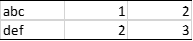
\includegraphics{pic_table.png}

Note: This was a png figure

}

\end{table}%

\texttt{@tbl-table1}: Table~\ref{tbl-table1} is a table that was
constructed in Excel, saved as figure, and reused in quarto. Notice that
the code \texttt{tbl-pos="H"} allows the table to be rendered close to
where the code was provided. Otherwise, in latex style, it would be
possitioned elsewhere.

Notice as well that after the ``table'' was declared, the first line
will correspond to the notes you add to your table, and the second one
to the title of the table.

\subsection{Adding Mark down as
tables}\label{adding-mark-down-as-tables}

Something that has been standard in quarto is to utilize markdown code
to create tables. Adding them is straigh forward, as you simply need to
include the code in text. But, to keep formatting standard, I will use
the same syntax as earlier.

The main difference is the use of \texttt{include} code. One advantage
is that the main document would be cleaner. Also, when using Markdown
tables, those will be rendered wherever the code was added.

\begin{Shaded}
\begin{Highlighting}[]
\NormalTok{::: \{\#tbl{-}table2\}}

\NormalTok{\{\{\textless{} include md\_table.md \textgreater{}\}\}}

\NormalTok{Note: Random note}

\NormalTok{Table using Markdown code}

\NormalTok{:::}
\end{Highlighting}
\end{Shaded}

\begin{longtable}[]{@{}lll@{}}

\caption{\label{tbl-table2}Table using Markdown code}

\tabularnewline

\toprule\noalign{}
Column 1 & Column 2 & Column 3 \\
\midrule\noalign{}
\endhead
\bottomrule\noalign{}
\endlastfoot
Row 1 & Data & Data \\
Row 2 & Data & Data \\
Row 3 & Data & Data \\

\end{longtable}

Note: Random note

\texttt{@tbl-table2} can be used to refer to Table~\ref{tbl-table2}.

\subsection{Adding HTML as tables}\label{adding-html-as-tables}

Using HTML code is just as simple. However, one needs to make sure that,
in addition to the code that produces the table of interest, that table
is fenced using
\texttt{\textasciigrave{}\textasciigrave{}\textasciigrave{}\{=html\}}.
This makes a explicit request to interpret HTML code as RAW code.

As with the example with a picture code, however, you may want to use
\texttt{tbl-pos="H"} to render the table where you want.

\begin{Shaded}
\begin{Highlighting}[]
\NormalTok{::: \{\#tbl{-}table3 tbl{-}pos="H"\}}
\InformationTok{\textasciigrave{}\textasciigrave{}\textasciigrave{}\{=html\}}
\InformationTok{\{\{\textless{} include html\_table.html \textgreater{}\}\}}
\InformationTok{\textasciigrave{}\textasciigrave{}\textasciigrave{}}

\NormalTok{Note: Random note}

\NormalTok{Table using HTML code  }
\NormalTok{:::}
\end{Highlighting}
\end{Shaded}

\begin{longtable}[]{@{}lll@{}}

\caption{\label{tbl-table3}Table using HTML code}

\tabularnewline

\toprule\noalign{}
\endhead
\bottomrule\noalign{}
\endlastfoot
Column 1 & Column 2 & Column 3 \\
Row 1 & Data & Data \\
Row 2 & Data & Data \\
Row 3 & Data & Data \\

\end{longtable}

Note: Random note

\texttt{@tbl-table3} is used now to render Table~\ref{tbl-table3}.

\subsection{Adding Latex as tables}\label{adding-latex-as-tables}

Last but not least, Latex tables. They can also be rendered using the
same strategy as before. Perhaps one important difference is that you
could modify the Latex code directly to decide where to position the
tables.

\begin{Shaded}
\begin{Highlighting}[]
\NormalTok{::: \{\#tbl{-}table4 tbl{-}pos="H"\}}
\NormalTok{\{\{\textless{} include latex\_table.tex \textgreater{}\}\} }

\NormalTok{Note: Random note}

\NormalTok{Table using Latex code}
\NormalTok{:::}
\end{Highlighting}
\end{Shaded}

\begin{table}[H]

\caption{\label{tbl-table4}Table using Latex code}

\centering{

    \centering
    \begin{tabular}{|c|c|c|}
    \hline
    \textbf{Column 1} & \textbf{Column 2} & \textbf{Column 3} \\
    \hline
    Row 1 & Data & Data \\
    \hline
    Row 2 & Data & Data \\
    \hline
    Row 3 & Data & Data \\
    \hline
    \end{tabular}

Note: Random note

}

\end{table}%

\texttt{@tbl-table4} is used to reference Table~\ref{tbl-table4}

\section{Adding References section}\label{adding-references-section}

to add reference section at the end of your document, you can use the
following code:

\begin{Shaded}
\begin{Highlighting}[]
\FunctionTok{\# References \{.unnumbered\}}

\NormalTok{::: \{\#refs\}}
\NormalTok{:::}
\end{Highlighting}
\end{Shaded}

The option \texttt{\{.unnumbered\}} request not to add a number to the
section. whereas the fenced code request to add the references in the
section of your choice.

\lipsum[1-4]

\section*{References}\label{references}
\addcontentsline{toc}{section}{References}

\phantomsection\label{refs}
\begin{CSLReferences}{1}{0}
\bibitem[\citeproctext]{ref-CameronTrivedi2013}
Cameron, A. C., and Trivedi, P. K. (2013). \emph{Regression analysis of
count data} (2nd ed.). Cambridge University Press.

\end{CSLReferences}

\newpage{}

\appendix
\pagenumbering{arabic}
\renewcommand{\thepage}{\thesection\arabic{page}}

\section{Appendix on how to add an
appendix}\label{appendix-on-how-to-add-an-appendix}

I find that adding an appendix requires two pieces of code. First, after
reference one may add \texttt{} to start a new page. And use the latex
code \texttt{\textbackslash{}appendix}, to start the appendix section.

Now, to re-start numnering, one needs to add
\texttt{\textbackslash{}setcounter\{page\}\{1\}} right after
\texttt{\textbackslash{}appendix}. However, if one wants to create new
pages for every appendix section, that is possible using the following
commands:

\begin{verbatim}
\pagenumbering{arabic}
\renewcommand{\thepage}{\thesection\arabic{page}}
\end{verbatim}

To add Appendix Figures and Tables, one can just create them as usual.

\subsection{Subsection Appendix}\label{subsection-appendix}

Just an example.

\lipsum[1-4]

\begin{table}[H]

\caption{\label{tbl-atable1}Appendix using Latex code}

\centering{

    \centering
    \begin{tabular}{|c|c|c|}
    \hline
    \textbf{Column 1} & \textbf{Column 2} & \textbf{Column 3} \\
    \hline
    Row 1 & Data & Data \\
    \hline
    Row 2 & Data & Data \\
    \hline
    Row 3 & Data & Data \\
    \hline
    \end{tabular}

Note: Random note

}

\end{table}%

\lipsum[2-4]

\newpage{}

\setcounter{page}{1}

\section{second appendix}\label{second-appendix}

Or a Second picture

\begin{table}[H]

\caption{\label{tbl-atable2}Appendix using Latex code}

\centering{

    \centering
    \begin{tabular}{|c|c|c|}
    \hline
    \textbf{Column 1} & \textbf{Column 2} & \textbf{Column 3} \\
    \hline
    Row 1 & Data & Data \\
    \hline
    Row 2 & Data & Data \\
    \hline
    Row 3 & Data & Data \\
    \hline
    \end{tabular}

Note: Random note

}

\end{table}%

\lipsum[1-2]

\subsection{sub appendix}\label{sub-appendix}

\lipsum[1-4]



\end{document}
